\documentclass[a4paper,12pt]{article}
\usepackage[utf8]{inputenc}
\usepackage[french]{babel}
\usepackage[T1]{fontenc}
\usepackage[top=2cm,bottom=2cm,left=2cm,right=2cm]{geometry}
\usepackage{graphicx}
\usepackage{wrapfig}
\usepackage{url}

\begin{document}

\begin{titlepage}
	\begin{center}
		\Large{Année universitaire 2016-2017}\\
		\Large{Université de Caen Basse-Normandie}\\[1cm]
		
		\huge{Rapport sur la numérotation des lignes sur l'éditeur}\\
		\vspace{3cm}
		
		Thomas Lécluse
		
	\normalsize{\textit{ ~ L2 Informatique}}\\
		\medskip
		\vspace{2cm}
				
	\end{center}
\end{titlepage}

\tableofcontents
\newpage

\section{Insertion dans l'interface graphique}

	L'objet que nous utilisons pour afficher et éditer le code est un QTextEdit de QT. Il ne possède pas de méthode pour afficher les numéros de lignes, et il n'y a pas d'autres alternatives à celui-ci pour faire cela non plus.\\
	
	Il nous fallait donc un autre élément, afin d'afficher les numéros de lignes qui serait placé sur le côté, nous avons choisi le côté droit.
	
		\begin{figure}[h!]
			\begin{center}
				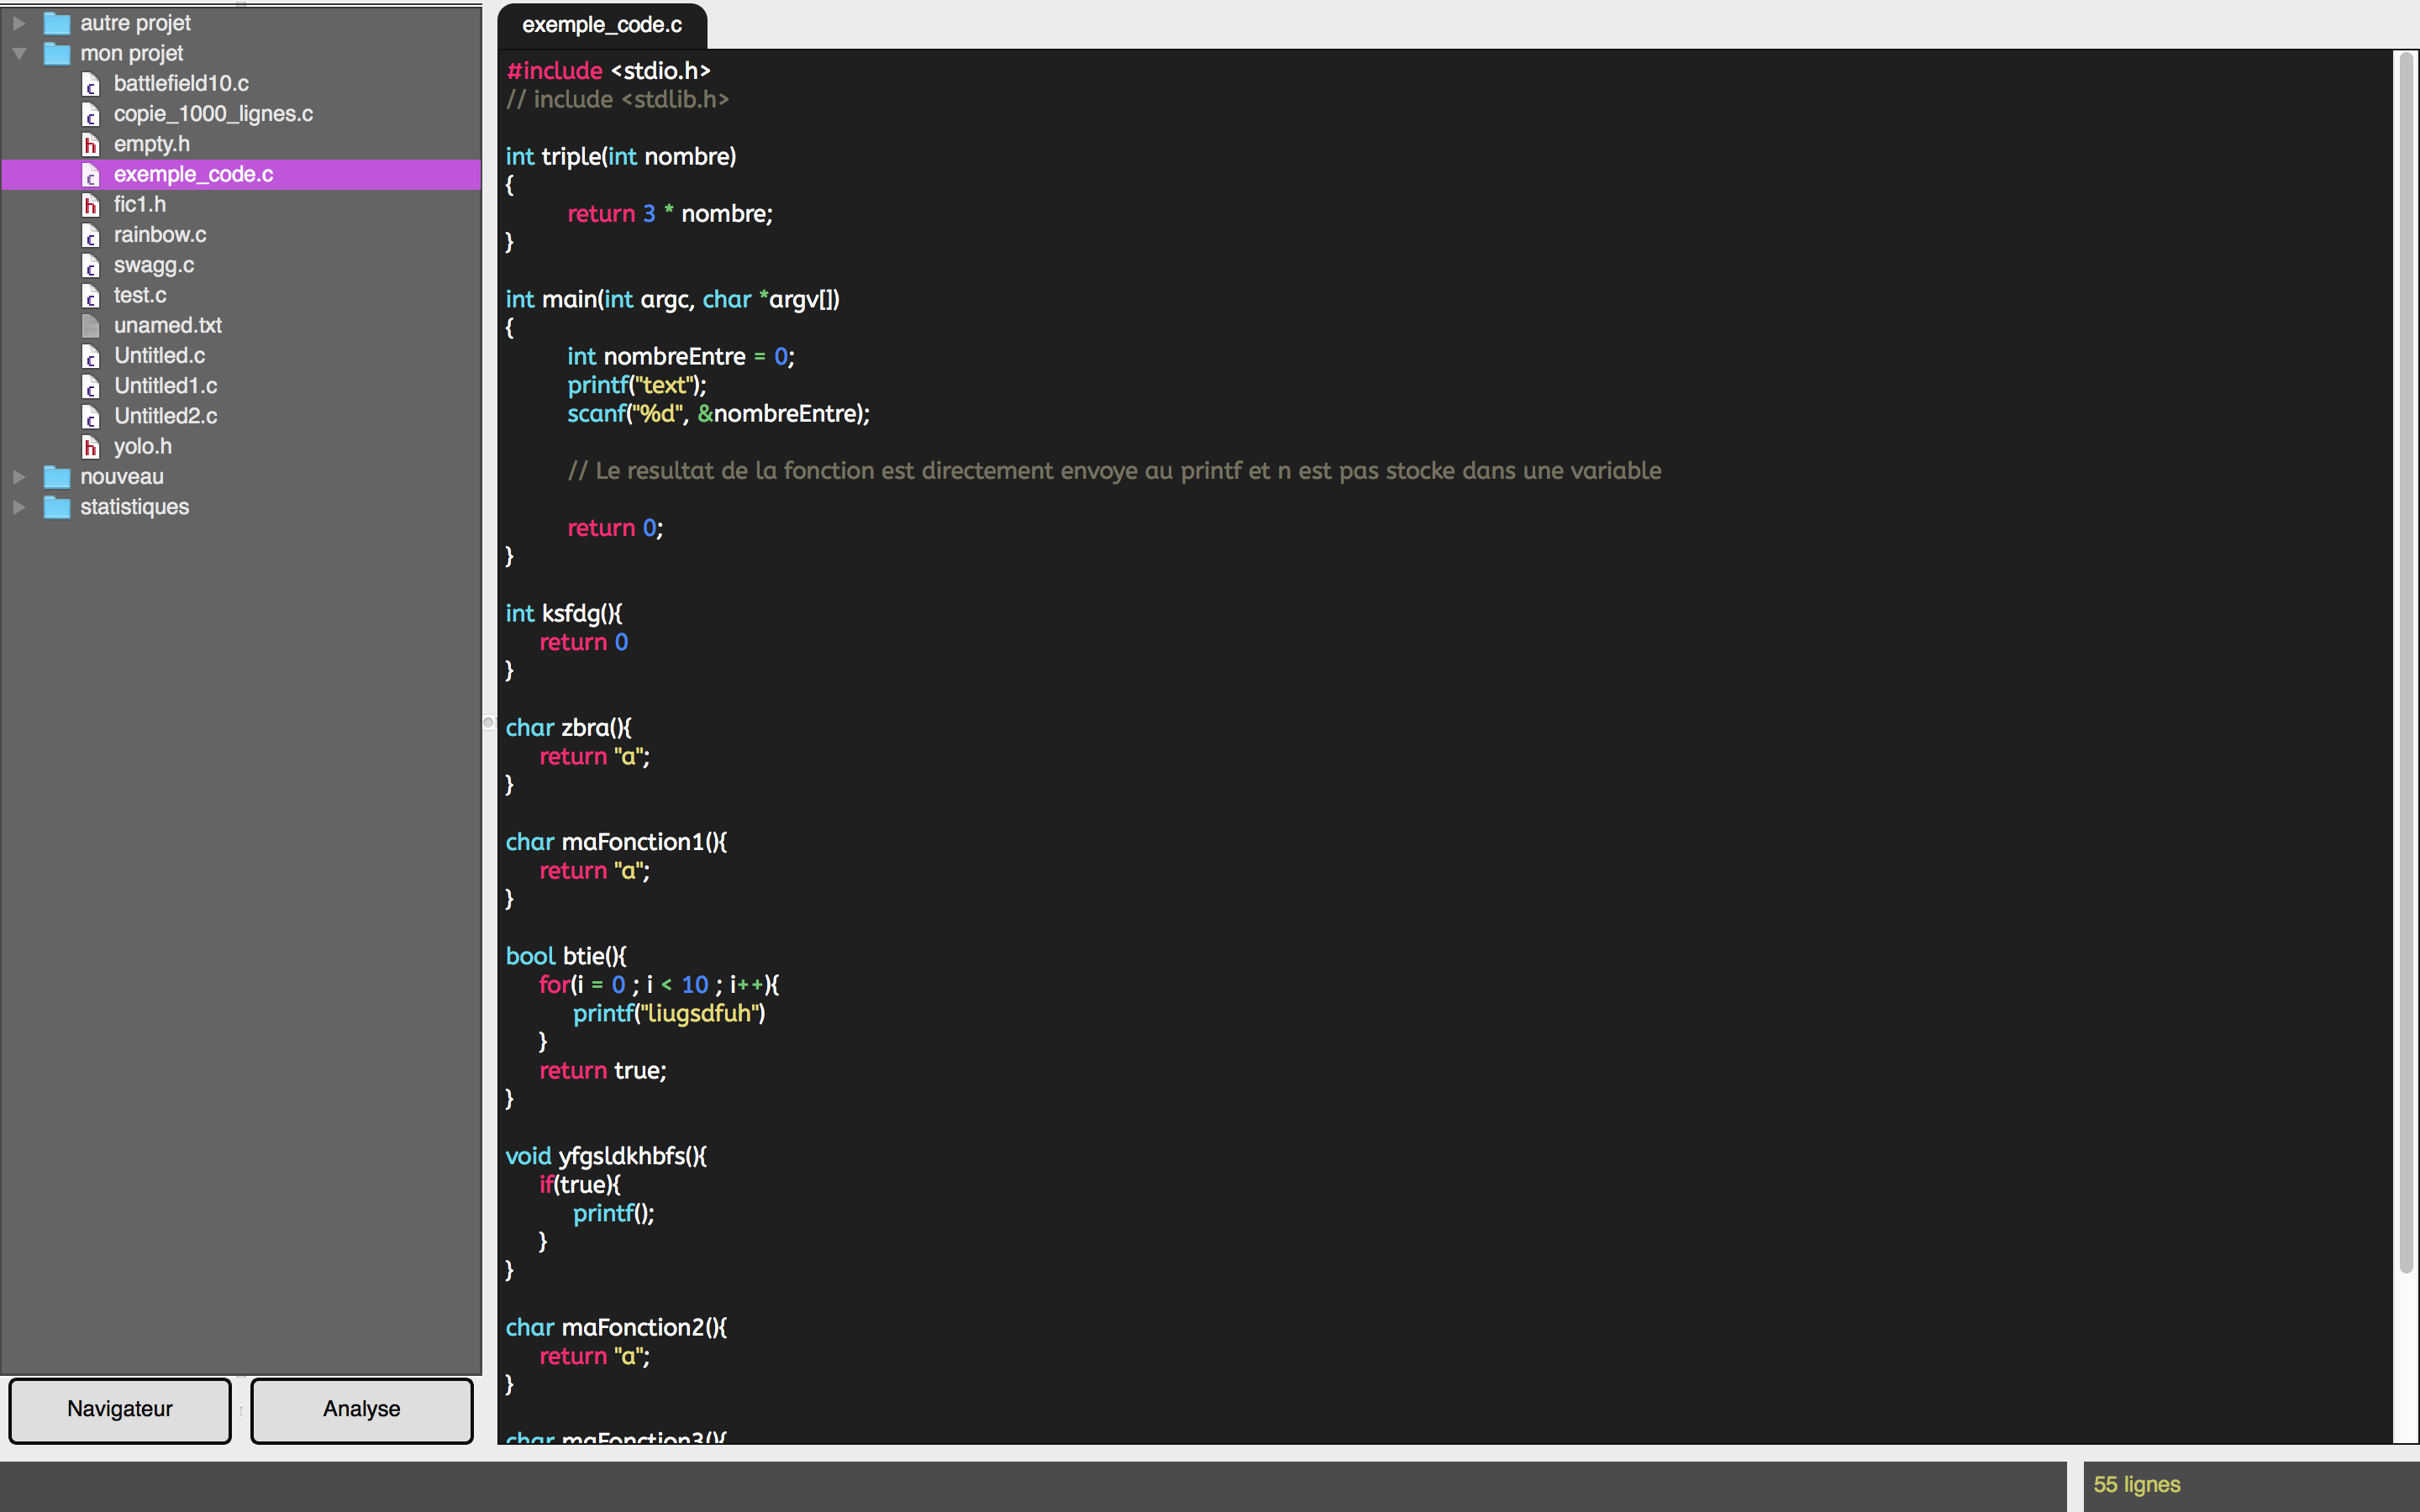
\includegraphics[scale=0.25]{images/avant}
				\caption{Sans la barre de numérotation des lignes}
			\end{center}
		\end{figure}
		
		\begin{figure}[h!]
			\begin{center}
				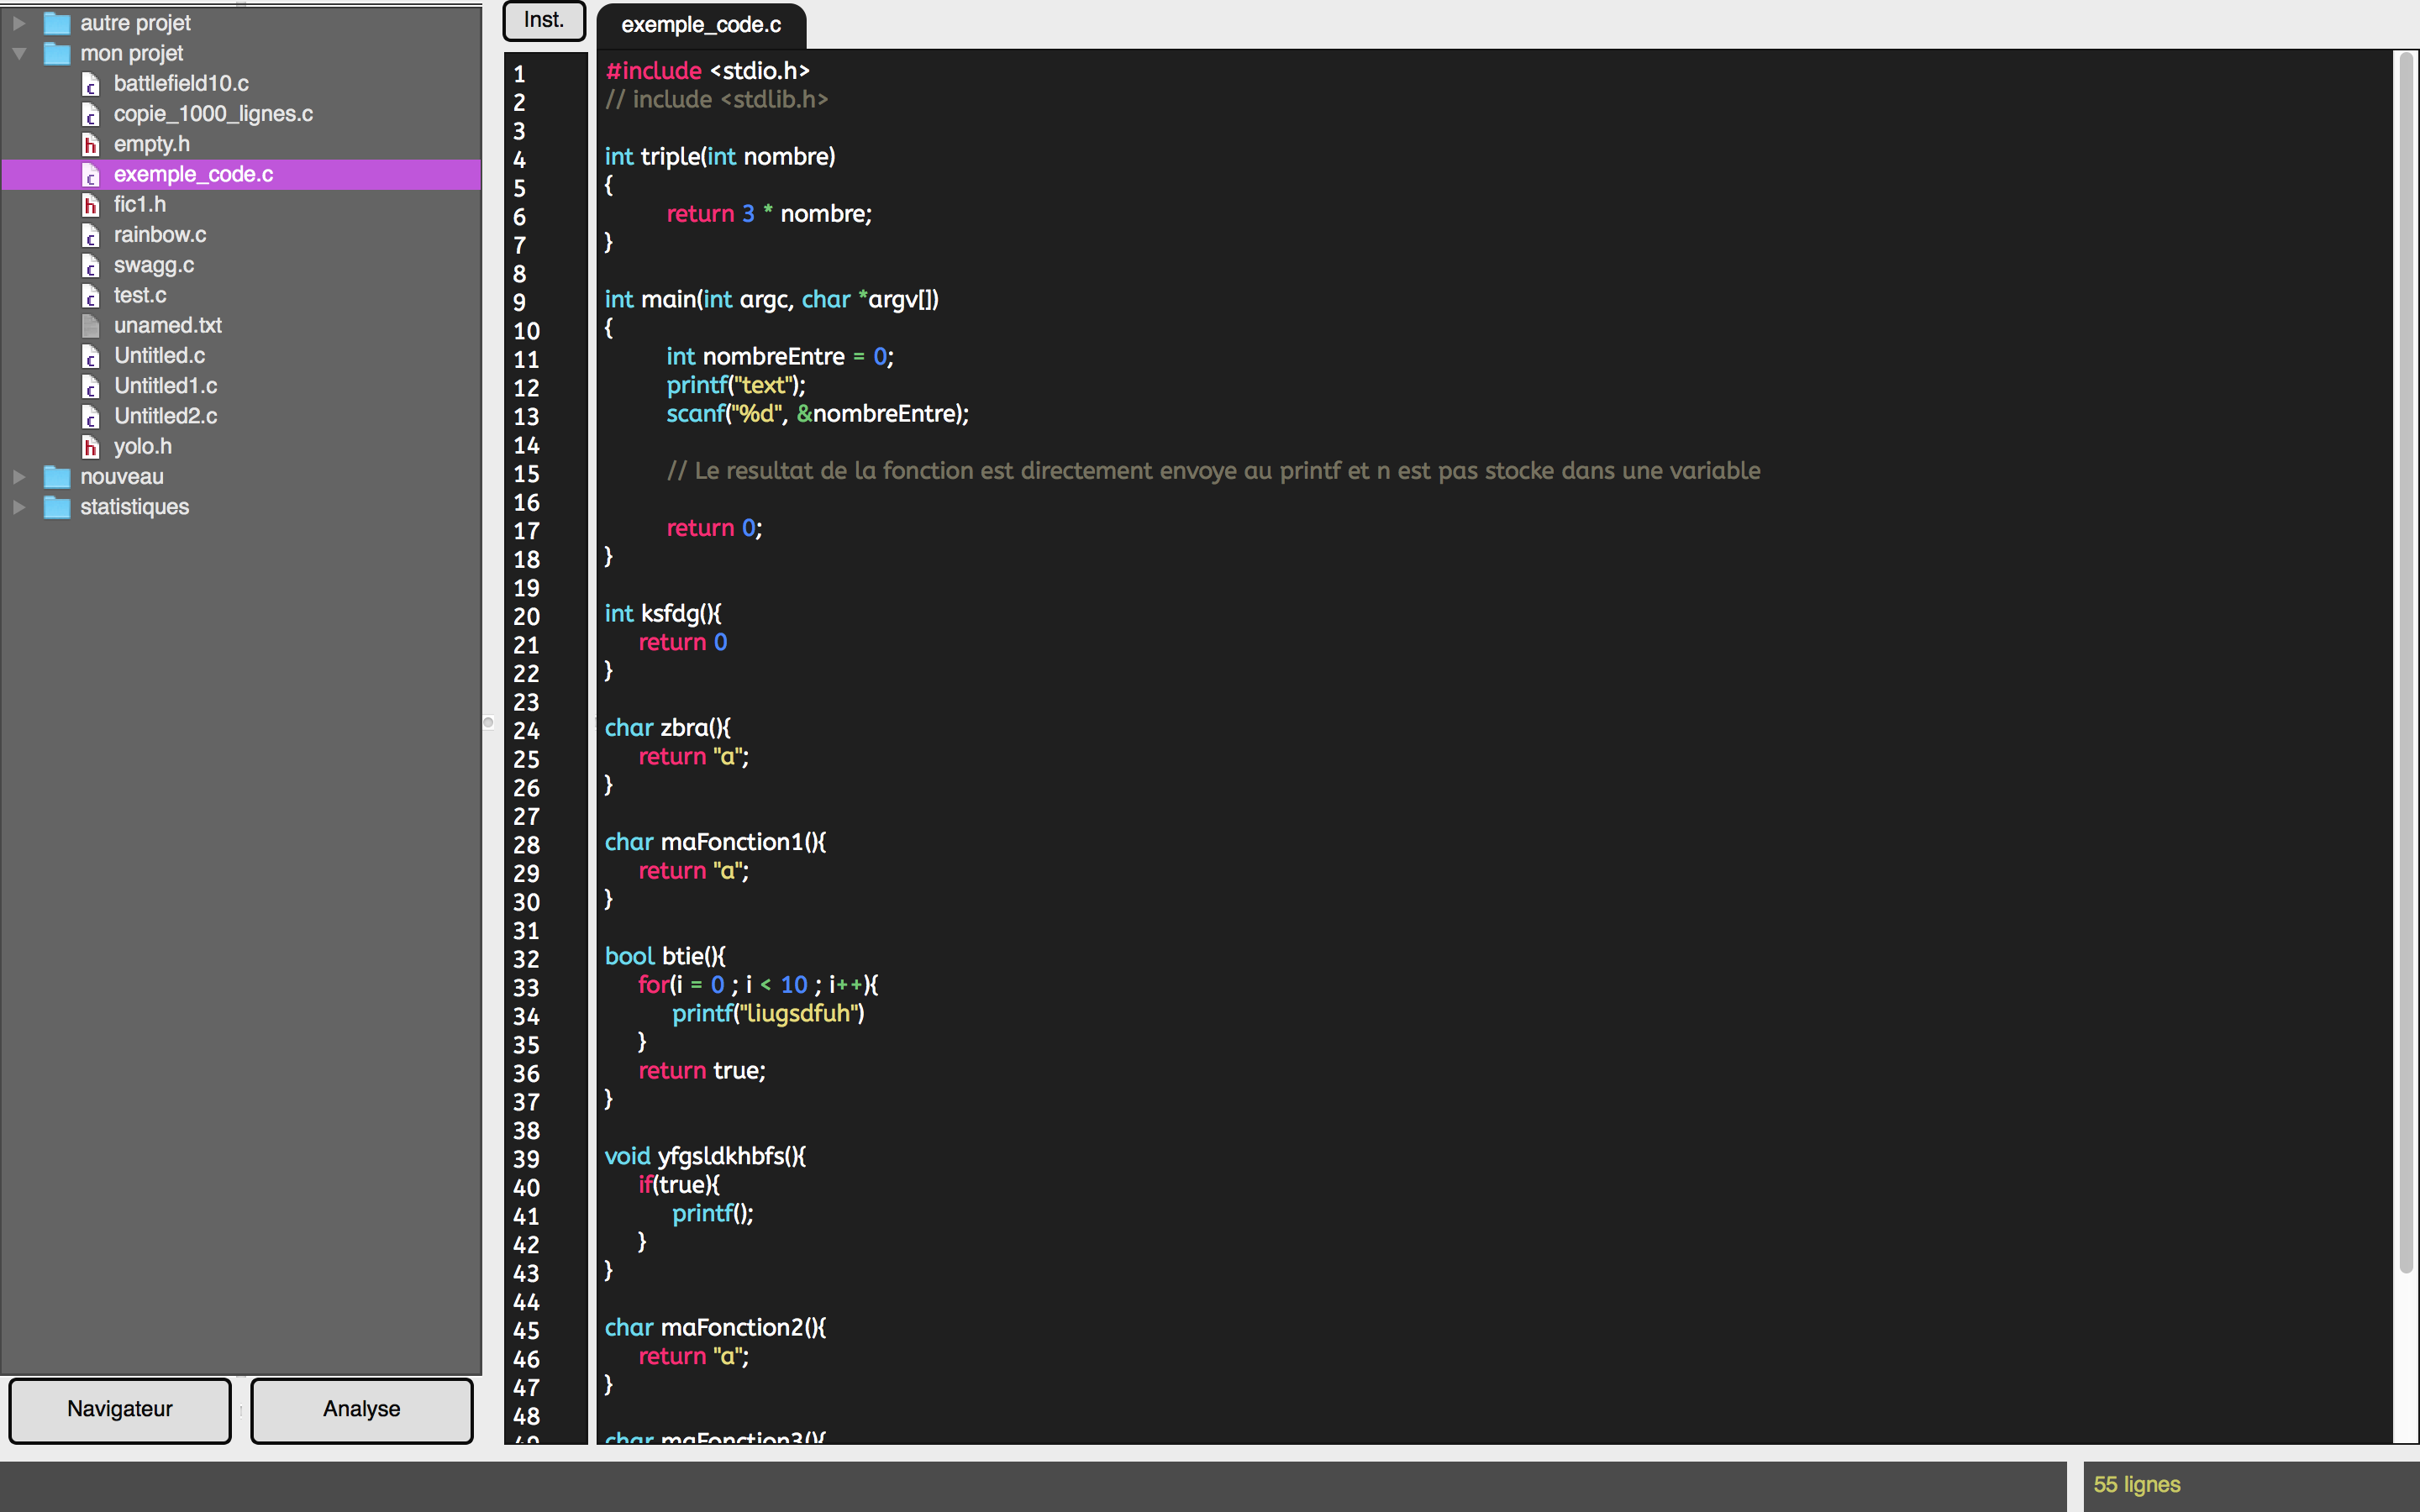
\includegraphics[scale=0.25]{images/apres}
				\caption{Avec la barre de numérotation des lignes}
			\end{center}
		\end{figure}
		
	L'utilisateur peut choisir d'afficher ou non cette barre.
	
		\begin{figure}[h!]
			\begin{center}
				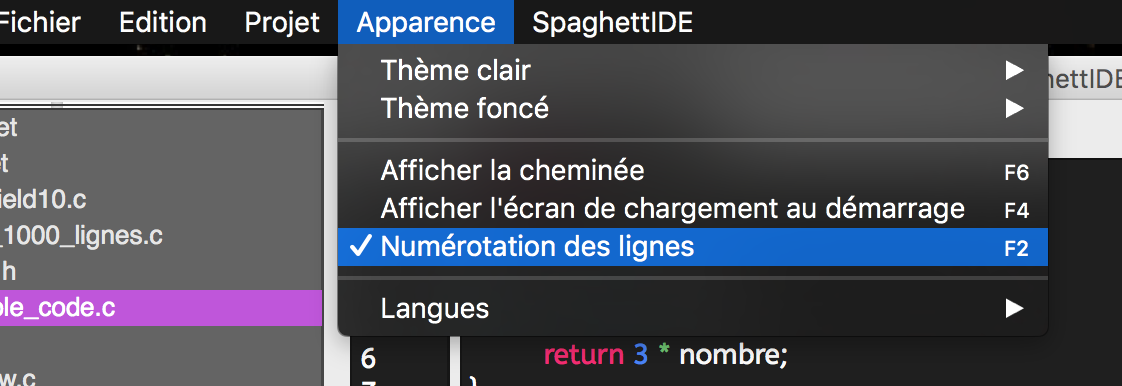
\includegraphics[scale=0.8]{images/menu}
				\caption{Dans le menu apparence}
			\end{center}
		\end{figure}
		
\section{Comment faire ?}

	La difficulté n'était pas d'afficher une barre avec des numéros dedans, ni de récupérer le nombre de lignes, car nous avons une méthode pour cela. La difficulté était de syncroniser le défilement des deux éléments (widgets).
	
	\subsection{Les signaux}
	
		Une première idée était d'intercepter les signaux émis par les éléments respectifs, afin d'envoyer à l'autre élément le décalage à effectuer. Le problème était qu'il n'y a pas de moyens de connaître la première ligne affichée sur le QTextEdit du code. On ne peut pas donc savoir de combien on décale d'autre façon d'incrémenter et de décrémenter "manuellement" une  variable en fonction du défilement que l'on effectue.\\
		
		Le soucis est que c'est très compliqué (pas réussi) de récupérer le nombre de lignes que l'on a décalé lors du défilement. La seule chose qu'on arrive à récupérer est un delta qui correspond à la vitesse de défilement que l'utilisateur a fait avec la molette de sa souris ou de son pad. Cela nous donne juste le sens du défliement.\\
		
		Il a fallu chercher une autre solution, plus propre et plus efficace.
		
	\subsection{Surcharger les méthodes originales}
		
		Lorsque l'on fait un défilement avec la molette de souris ou le pad \textbf{uniquement}, la méthode appelée sur le QTextEdit est le "wheelEvent(e)" où "e" est l'évenement utilisé par QT pour effectuer le défilement.\\
		
		Le principe consiste à appeler la fonction d'origine ainsi que celle de l'autre objet avec le même argument "e" lorsque la méthode "wheelEvent()" est appelée.
		
		\newpage		
		
		\begin{figure}[h!]
			\begin{center}
				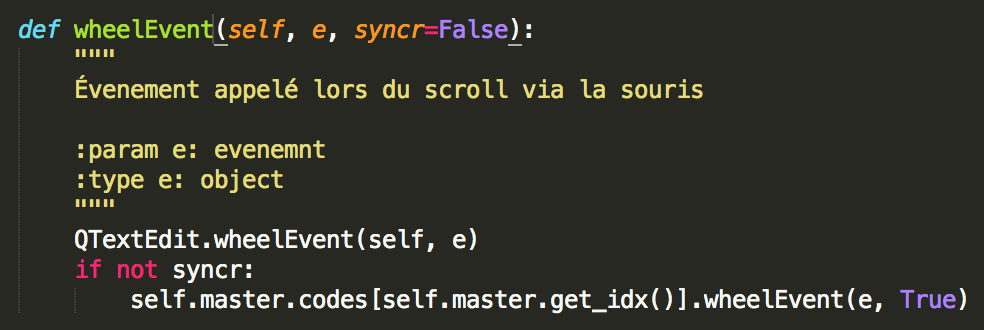
\includegraphics[scale=0.9]{images/wheel_lines}
				\caption{Méthode de l'objet contenant la numérotation des lignes}
			\end{center}
		\end{figure}
		
		
		Ici, "self.master.codes" désigne la liste des onglets de codes ouverts, et "self.master.get\_idx()" retourne l'indice de l'onglet courant. On appelle donc la méthode "wheelEvent()" de l'onglet courant lorsque l'on fait défiler la liste de numérotation des lignes. L'argument booléen sert à dire qu'il ne faut pas rappeler la méthode "wheelEvent()" car sinon on rentrerait dans une boucle infinie.\\
		
		\begin{figure}[h!]
			\begin{center}
				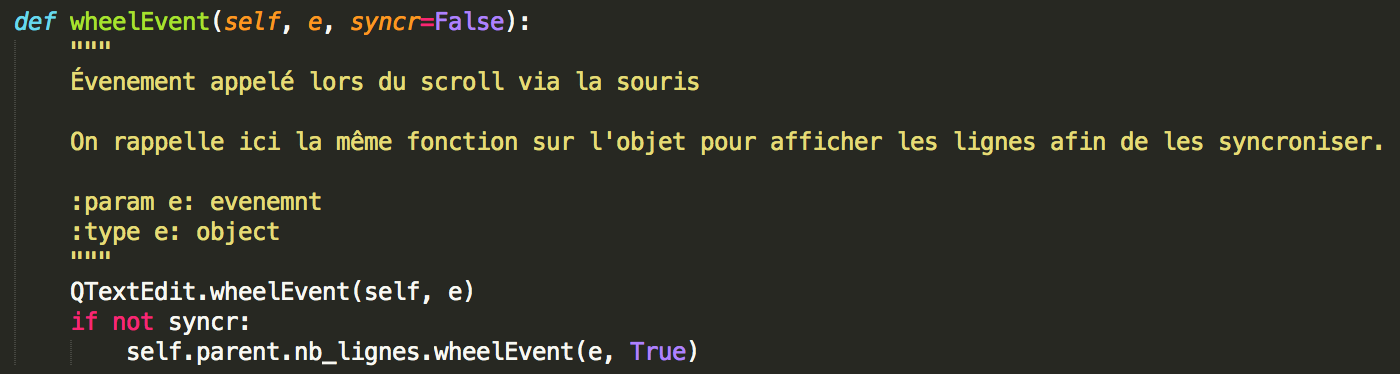
\includegraphics[scale=0.7]{images/wheel_code}
				\caption{Méthode de l'objet contenant le code}
			\end{center}
		\end{figure}
		
		"self.parent.nb\_lignes" désigne l'objet contenant la numérotation des lignes, on y appelle donc la méthode "wheelEvent()" avec les même arguments. Et toujours l'argument empêchant la boucle infinie.\\
		
		
		Nous arrivons ainsi à syncroniser les deux éléments lors du défilement de l'un comme de l'autre avec la souris ou le pad.
		
		Le bon fonctionnement de cette fonctionnalité est difficile à montrer dans un rapport, mais voici tout de même un exemple :
		
		\begin{figure}[h!]
			\begin{center}
				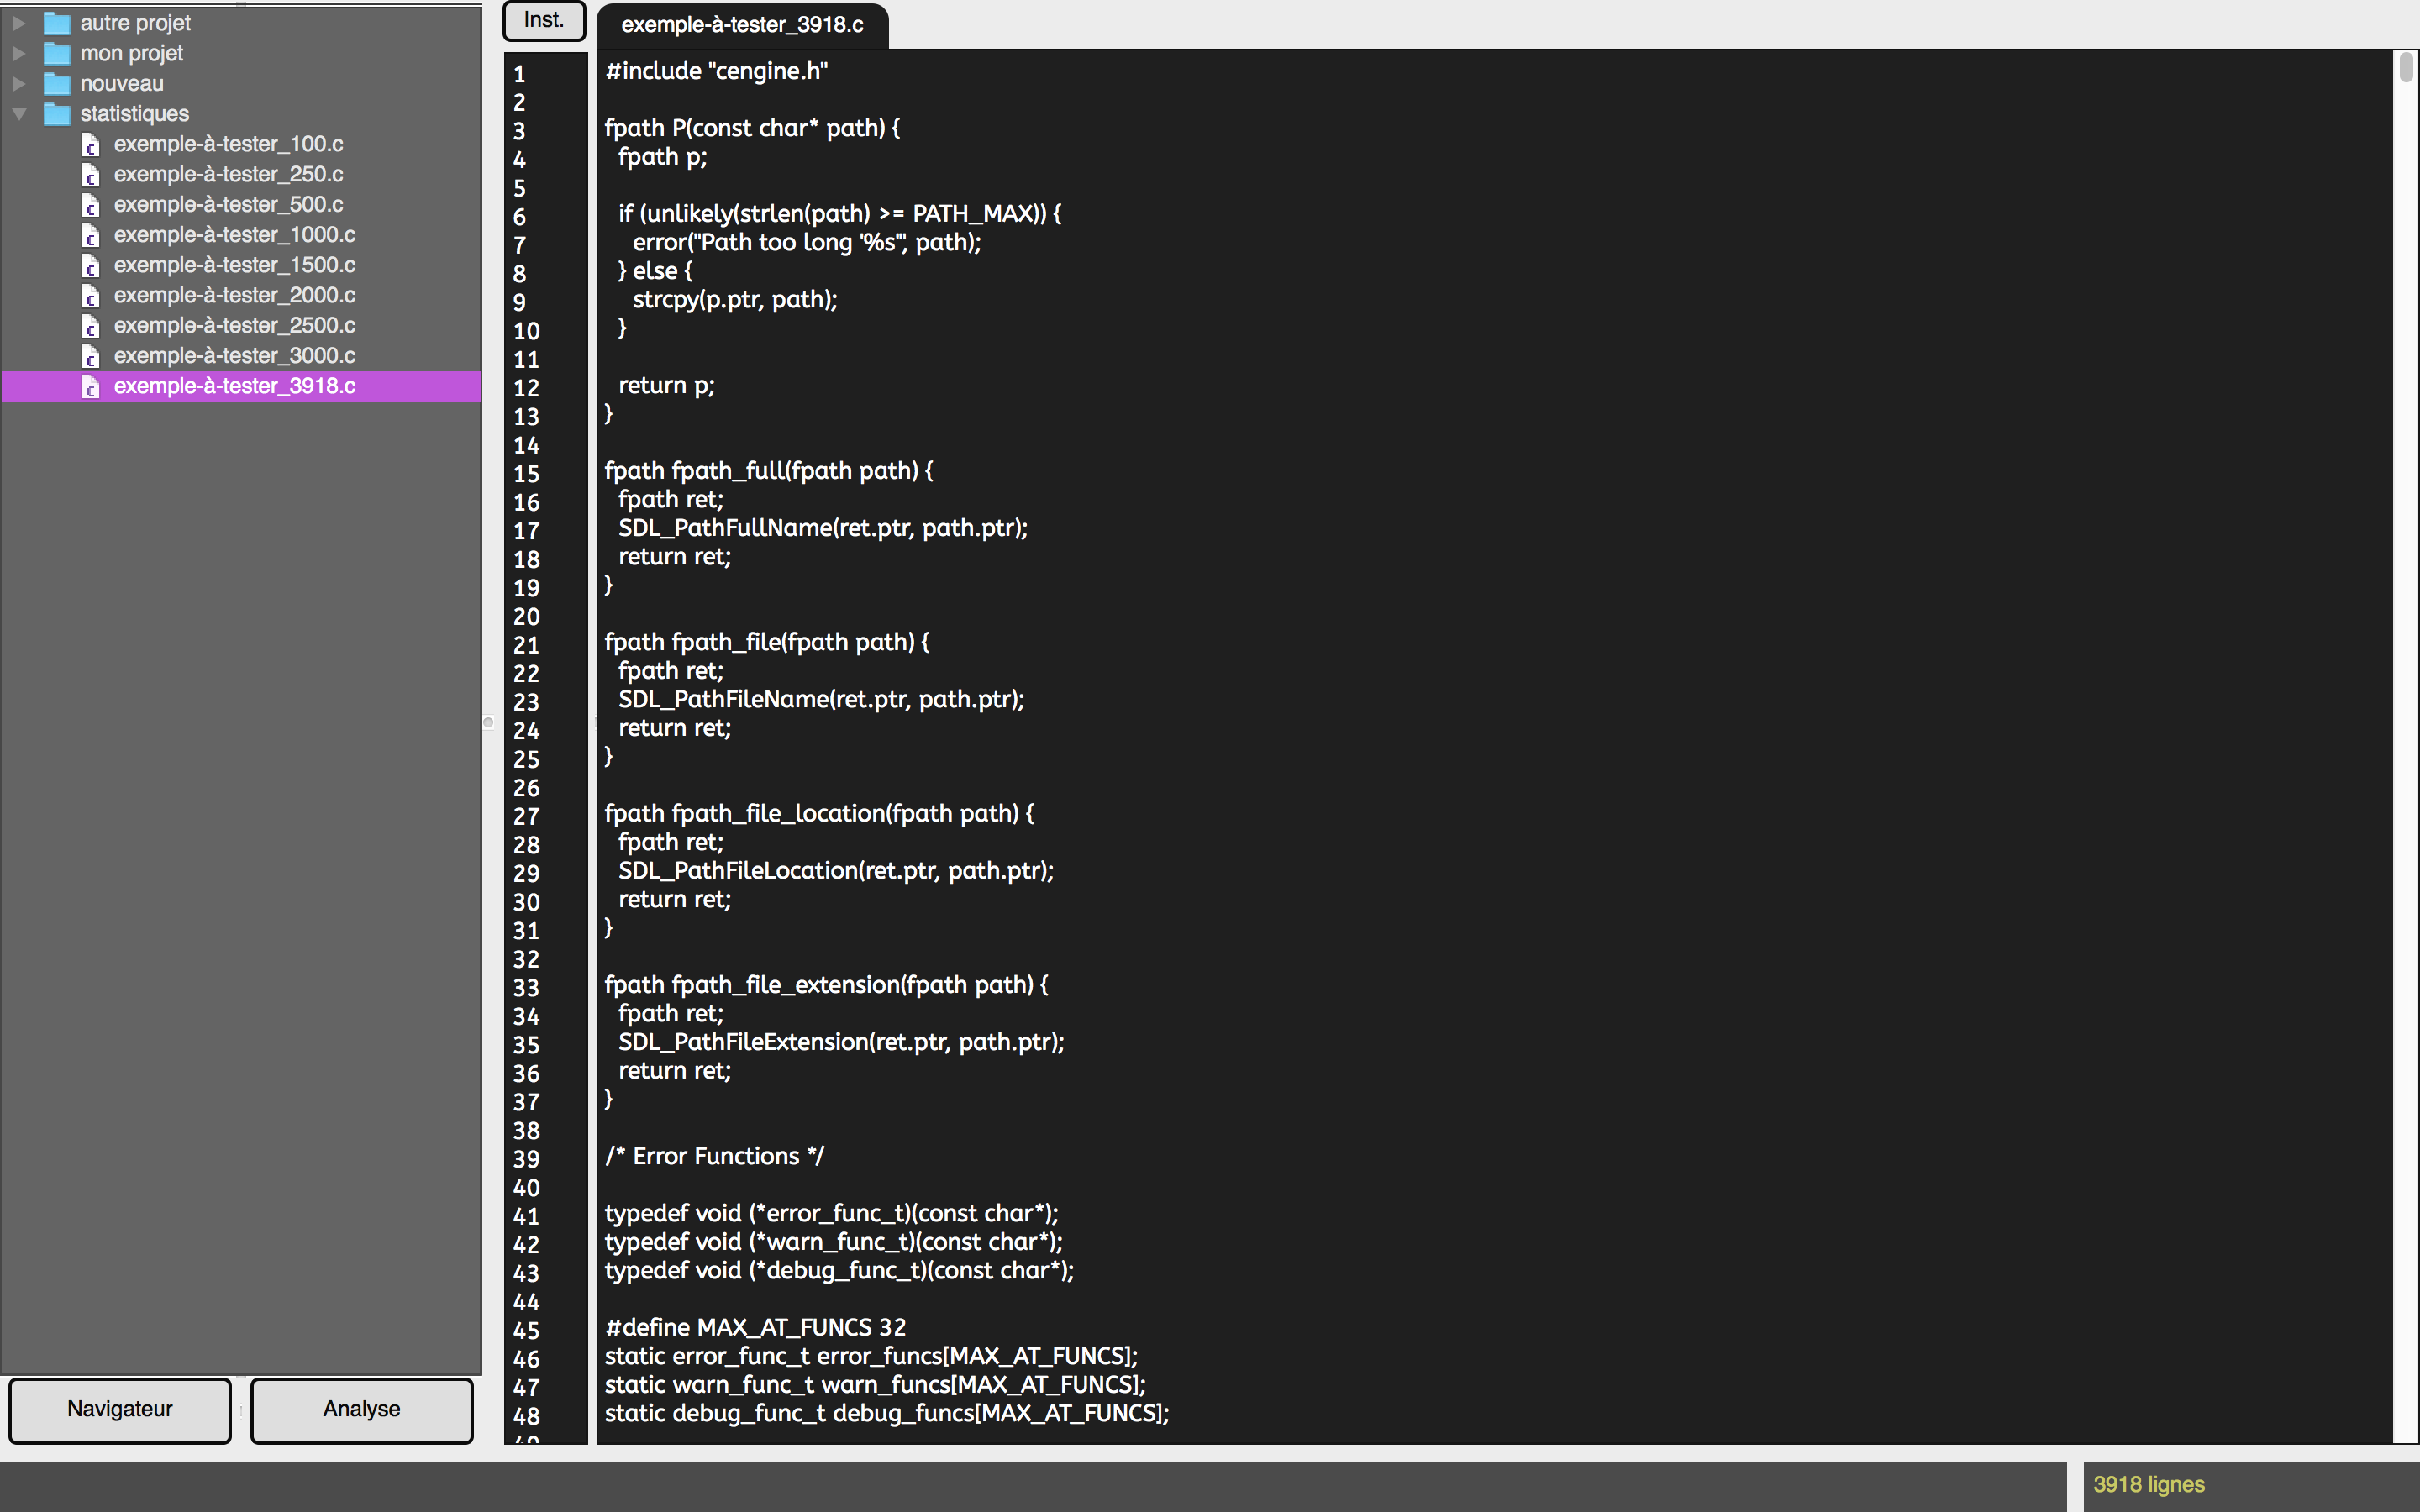
\includegraphics[scale=0.2]{images/l1}
				\caption{Premier exemple : haut du code, bien en face des numéros}
			\end{center}
		\end{figure}
		
		\begin{figure}[h!]
			\begin{center}
				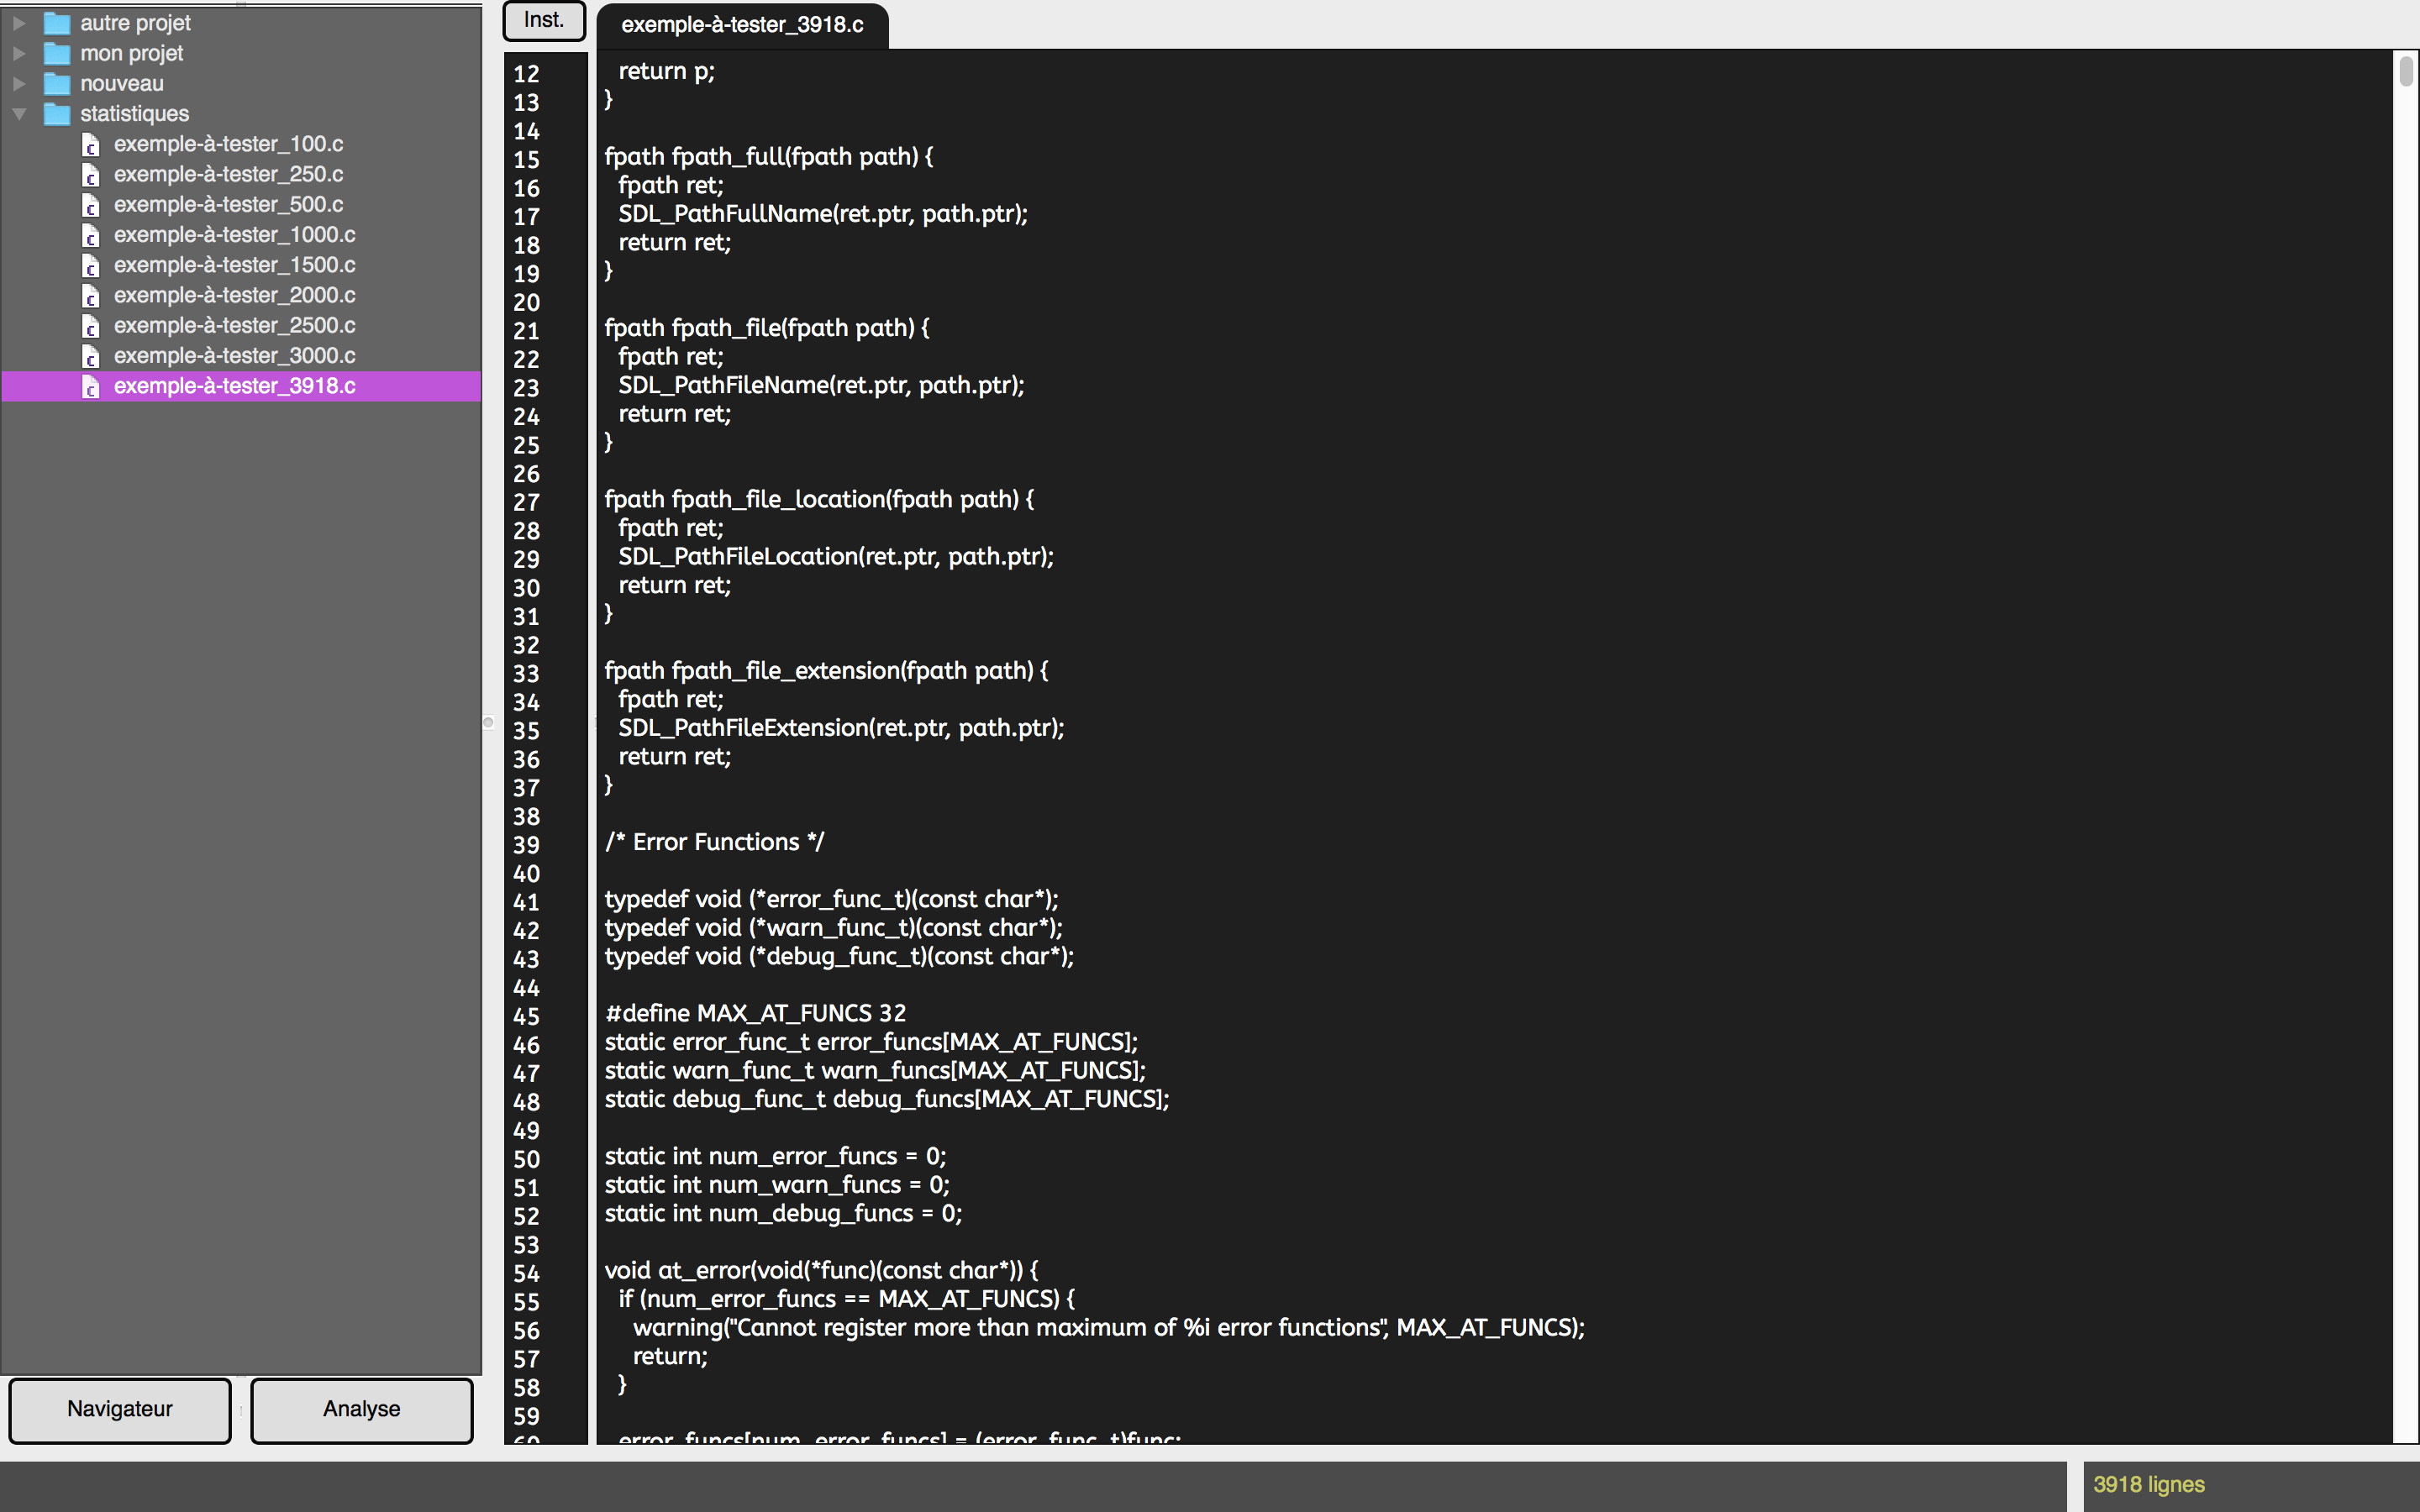
\includegraphics[scale=0.2]{images/l2}
				\caption{Deuxième exemple : les lignes sont toujours en face du code correspondant}
			\end{center}
		\end{figure}
	
		\begin{figure}[h!]
			\begin{center}
				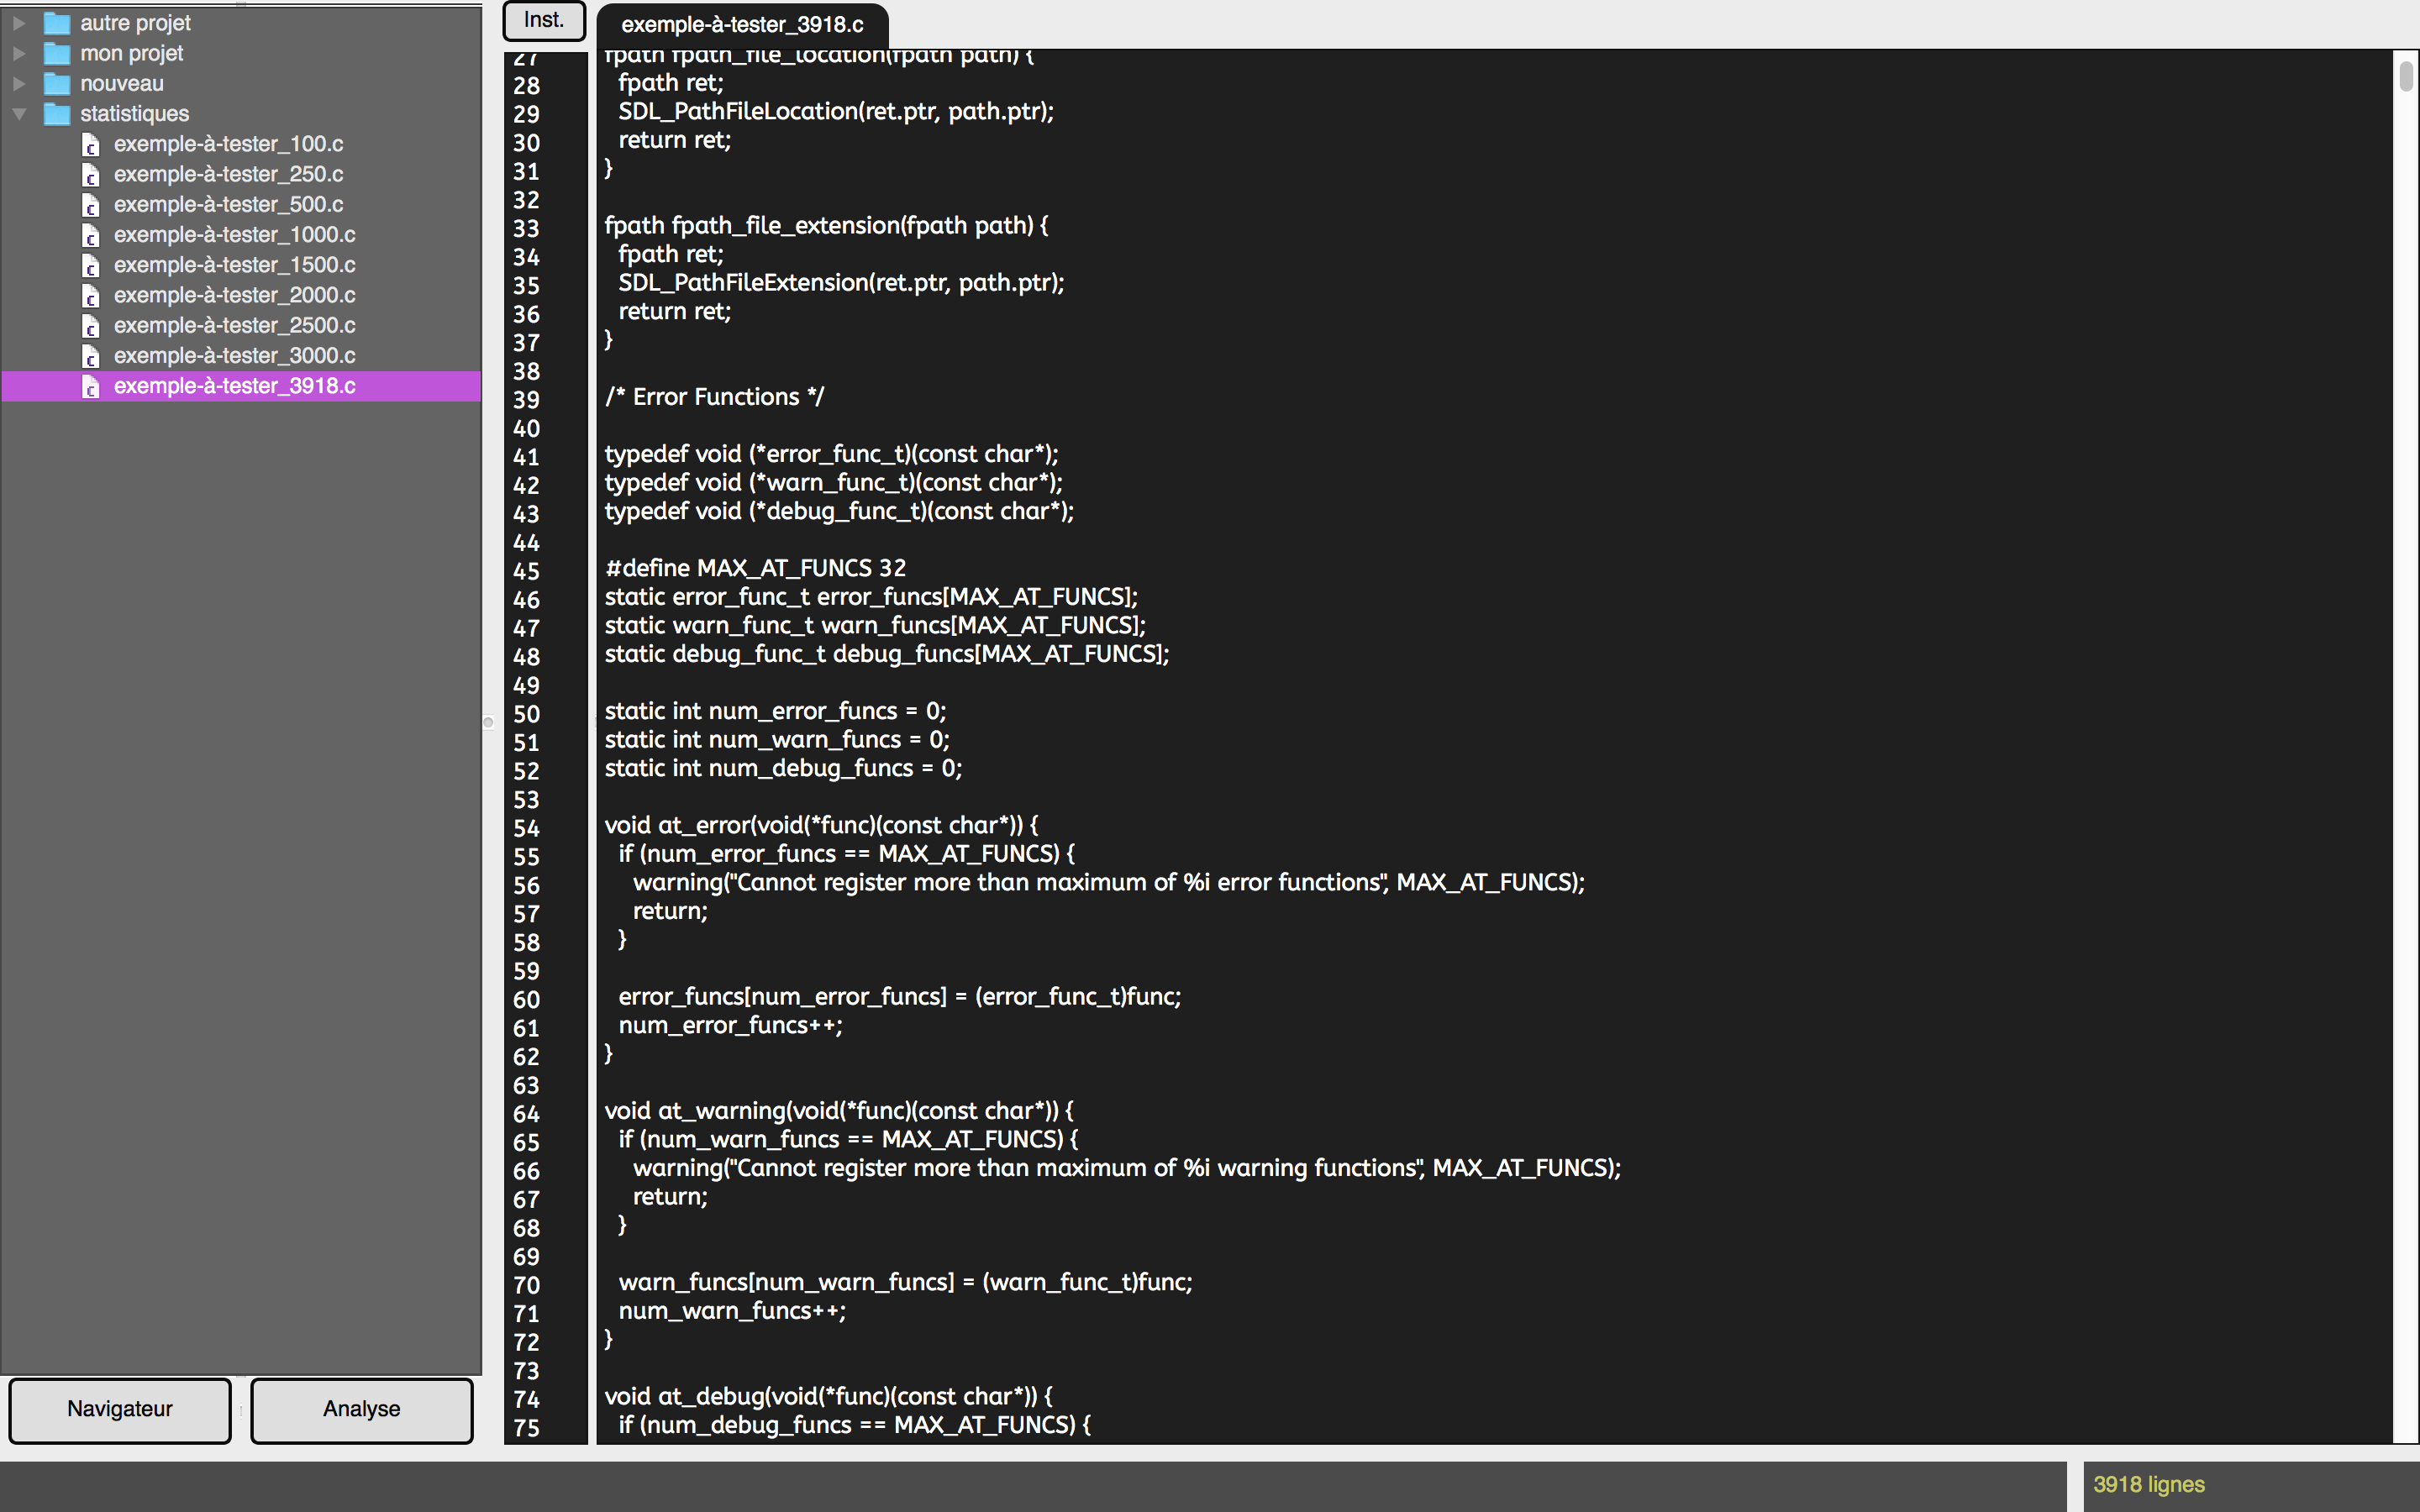
\includegraphics[scale=0.2]{images/l3}
				\caption{Dernier exemple : même si la moitié d'une ligne est affichée (en haut), la numérotation est toujours alignées}
			\end{center}
		\end{figure}
		
\newpage
		
\section{Pour finir}

	Néanmoins, lorsque le texte affiché est défilé à l'aide des flèches, la méthode "wheelEvent()" n'est pas appelée. Il va donc falloir trouver un moyen de syncroniser tout de même ces éléments.
		
		
		


\end{document}